% !TeX root = main.tex

\section{Measure of Center and Variation}

\hypertarget{median-quartiles-interquartile-range-and-outliers}{%
\subsection{Median, Quartiles, Interquartile Range and
Outliers}\label{median-quartiles-interquartile-range-and-outliers}}

\begin{itemize}
\item
  The three \textbf{quartiles}, \(Q_1\), \(Q_2\), and \(Q_3\) are
  numbers in an ordered data set that divide the data set into four
  equal parts. The second quartile is known as the \textbf{median}.
\item
  \textbf{Interquartile Range (IQR for short)} is the measure of
  variation when using the median to measure center. It is defined as
  the difference of the third and the first quartiles:
  \(\text{IQR}=Q_3-Q_1\).
\item
  When the center and the spread are measured by the median and the IQR,
  a value in the data is considered an \textbf{outlier} if the value is

  \begin{itemize}
  \item
    less than the lower fence
    \(\text{fence}_{lower}=Q_1 - 1.5 \cdot \text{IQR}\) or
  \item
    greater than the upper fence
    \(\text{fence}_{upper}=Q_3 + 1.5 \cdot \text{IQR}\).
  \end{itemize}

  \textbf{Note:} An outlier in this definition is also called a
  \textbf{mild outlier}. An outlier that is less than the extreme lower
  fence \(\text{extreme fence}_{lower}=Q_1 - 3 \cdot \text{IQR}\) or
  greater than the extreme upper fence
  \(\text{extreme fence}_{upper}=Q_3 + 3 \cdot \text{IQR}\) is also
  called \textbf{extreme outlier}.
\item
  The minimum, \(Q_1\), \(Q_2\), \(Q_3\) and maximum are known as the
  ``\textbf{five-number summary}'' of the data set.
\item
  The difference of maximum and minimum is called the \textbf{range}.
\end{itemize}

\begin{example}

Find the median, quartiles, IQR and outliers (if they exist) of the
sample height of 15 trees.

70, 65, 63, 72, 81, 83, 66, 75, 80, 75, 79, 76, 76, 69, 75

\end{example}
\vspace*{8\baselineskip}

\begin{exercise}

Find the five-number summary, the IQR and the Range for the following
set of data.

2, 7, 7, 7, 10, 11, 14, 17, 18, 20

\end{exercise}
\vspace*{6\baselineskip}

\hypertarget{box-plot}{%
\subsection{Box Plot}\label{box-plot}}

\begin{itemize}
\item
  A \textbf{box plot} shows a ``five-number summary'' of the data set.
  It contains a box, two whiskers and dots (for outliers).
\item
  To create the boxplot for a distribution,

  \begin{itemize}
  \item
    Draw a box from \(Q_1\) to \(Q_3\).
  \item
    Draw a vertical line in the box at the median.
  \item
    Extend a tail from \(Q_1\) to the smallest value that is not an
    outlier and from \(Q_3\) to the largest value that is not an
    outlier.
  \item
    Indicate outliers with a solid dot.
  \end{itemize}
\end{itemize}

\begin{example}
  Create the boxplot for the ages of 32 best actor oscar winners
  (1970--2001).
  
  31, 32, 32, 33, 35, 36, 37, 37, 38, 38, 39, 40, 40, 40, 42, 42, 43, 43,
  45, 45, 46, 47, 48, 48, 51, 55, 55, 56, 60, 60, 61, 76
\end{example}
\vspace*{6\baselineskip}

\begin{exercise}

Based on the boxplot below, identify the 5 number summary (minimum,
lower quartile (Q1), median (Q2), upper quartile (Q3), maximum)
\begin{fullwidth}
  \begin{center}
    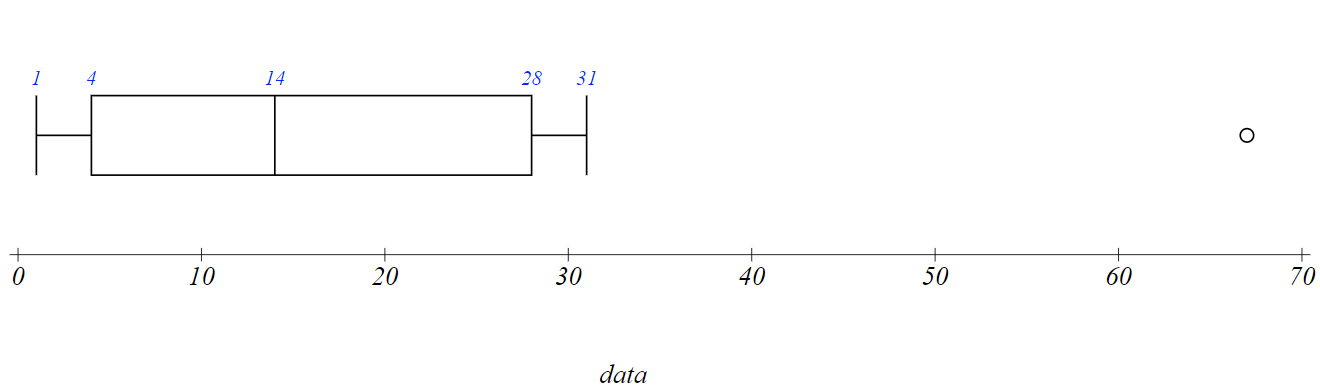
\includegraphics[width=0.9\linewidth]{Figures/Summary-Boxplot.png}
  \end{center}
\end{fullwidth}

\end{exercise}
\vspace*{6\baselineskip}

\hypertarget{mean-and-standard-deviation}{%
\subsection{Mean and Standard
Deviation}\label{mean-and-standard-deviation}}

\begin{itemize}
\item
  Sigma notation: in math, we denote the sum of values \(x_1\), \(x_2\),
  \(\dots\), \(x_n\) of a variable \(x\) by \(\sum\limits_{i=1}^n x_i\)
  or simply by \(\sum x\).
\item
  The \textbf{population mean} is \(\mu= \frac{\sum x}{N}\), where \(N\)
  is the \textbf{population size}, i.e the number of elements in the
  population.

  The notation \(\mu\) reads as mu.
\item
  The \textbf{sample mean} is \(\bar{x}=\frac{\sum{x}}{n}\), where \(n\)
  is the \textbf{sample size}. The notation \(\bar{x}\) reads as
  \(x\)--bar.
\end{itemize}

\begin{example}

Find the mean city mpg for a sample of 10 cars.

18, 21, 20, 21, 16, 18, 18, 18, 16, 20

\end{example}
\vspace*{6\baselineskip}

\hypertarget{weighted-mean}{%
\subsection{Weighted Mean}\label{weighted-mean}}

\begin{itemize}
\item
  The weighted mean of a set of numbers \(\{x_1, \dots, x_n\}\) with
  weights \(w_1\), \(w_2\), \ldots, \(w_n\) is defined as
  \[\frac{\sum w_ix_i}{\sum w_i}.\]
\item
  The mean of a frequency table is weighted mean
  \(\bar{x}=\frac{\sum f x}{n}\), where \(x\) is an element with
  frequency \(f\) and \(n\) is the sample size.
\end{itemize}

\begin{example}

In a course, the overall grade is determined in the following way: the
homework average counts for 10\%, the quiz average counts for 10\%, the
test average counts 50\% , and the final exam counts for 30\%. What's
the overall grade of the student who earned 92 on homework, 95 on
quizzes, 90 on tests and 93 on the final.

\end{example}
\vspace*{6\baselineskip}

\begin{exercise}

Find the average petal width for a sample of 10 iris followers.

0.2, 2.1, 0.2, 1.7, 2.3, 0.3, 1.2, 0.2, 1.8, 2.3

\end{exercise}
\vspace*{6\baselineskip}

\begin{exercise}

Find the mean and median from the dot plot of sepal length for a sample
of 10 iris flowers.

\begin{fullwidth}
  \begin{center}
    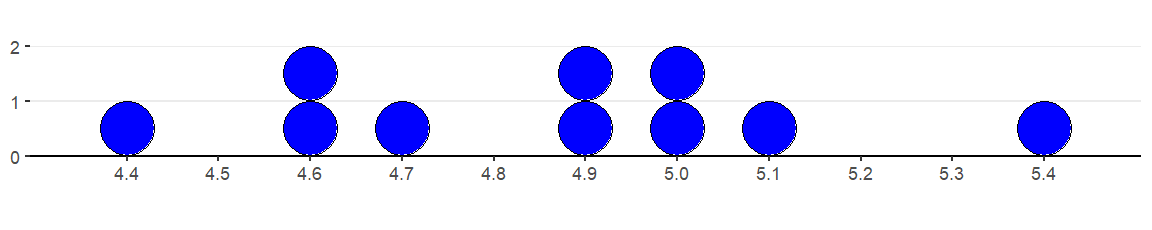
\includegraphics[width=0.8\linewidth]{Figures/MeanMedian-from-Dotplot.png}
  \end{center}
\end{fullwidth}

\end{exercise}
\vspace*{6\baselineskip}

\begin{exercise}

In a student's chemistry class, the final grade is based on six
categories.

The categories, grades, and weights are shown in this table.

\begin{longtable}[]{@{}lll@{}}
\toprule()
Category & Grade & Weight \% \\
\midrule()
\endhead
Test 1 & 46 & 20 \\
Test2 & 61 & 20 \\
Test 3 & 45 & 15 \\
Homework & 72 & 9 \\
Semester Project & 53 & 8 \\
Final Exam & 77 & 28 \\
\bottomrule()
\end{longtable}

Compute a weighted average to determine the student's overall final
grade in the course. Record the overall final grade below as a
percentage. Round accurately to two decimal places.

\end{exercise}
\vspace*{6\baselineskip}

\hypertarget{measure-of-variation-about-population-mean}{%
\subsection{Measure of Variation about Population
Mean}\label{measure-of-variation-about-population-mean}}

\begin{itemize}
\item
  The \textbf{deviation} of an entry \(x\) in a population data set is
  the difference \(x-\mu\), where \(\mu\) is the mean of the population.
\item
  The \textbf{population variance} of a population of \(N\) entries is
  defined as \[
    \text{VAR.P}=\sigma^2=\dfrac{\sum(x-\mu)^2}{N}.
  \]
\item
  The \textbf{population standard deviation} is \[
    \text{STDEV.P}=\sigma=\sqrt{\dfrac{\sum(x-\mu)^2}{N}}.
  \]
\end{itemize}

\hypertarget{measure-of-variation-about-sample-mean}{%
\subsection{Measure of Variation about Sample
Mean}\label{measure-of-variation-about-sample-mean}}

\begin{itemize}
\item
  The \textbf{deviation} of an entry \(x\) in a sample data set is the
  difference \(x-\bar{x}\), where \(\bar{x}\) is the mean of the sample.
\item
  The \textbf{sample variance} and \textbf{sample standard deviation}
  are defined similarly \[
    \text{VAR.S}=s^2=\dfrac{\sum(x-\bar{x})^2}{n-1}, \qquad
    \text{STDEV.S}=s=\sqrt{\dfrac{\sum(x-\bar{x})^2}{n-1}},
  \] where \(n\) is the sample size.
\item
  \textbf{Rounding rule:} for mean, variance and standard deviation, we
  keep at least one more digit than the accuracy of the data set.
\end{itemize}

\textbf{Note:} To measure the spread, one may also use the \textbf{mean
absolute deviation} \[MAD=\dfrac{\sum |x-\bar{x}|}{n}.\] However, the
standard deviation has better properties in applications.

\begin{example}

Find the mean and standard deviation ages of a sample of 32 best actor
oscar winners (1970--2001).

31, 32, 32, 33, 35, 36, 37, 37, 38, 38, 39, 40, 40, 40, 42, 42, 43, 43,
45, 45, 46, 47, 48, 48, 51, 55, 55, 56, 60, 60, 61, 76

\end{example}
\vspace*{6\baselineskip}

\begin{exercise}

A \emph{sample} of GPAs from ten students random chosen from a college
are recorded as follows.

1.90, 3.00, 2.53, 3.71, 2.12, 1.76, 2.71, 1.39, 4.00, 3.33

Find the standard deviation of this sample.

\end{exercise}
\vspace*{6\baselineskip}

\hypertarget{mean-and-standard-deviation-under-linear-transformation}{%
\subsection{Mean and Standard Deviation under Linear
Transformation}\label{mean-and-standard-deviation-under-linear-transformation}}

\begin{itemize}
\item
  When we increase values in a data set by a fixed number \(c\), the
  standard deviation of a data set won't change. However, the mean
  increases by \(c\) too.
\item
  When we multiple values in a data set by a factor \(k\), the mean and
  the standard deviation both scale by the factor \(k\).
\end{itemize}

\url{https://tinyurl.com/6vrp7ze8}

\hypertarget{effect-of-changes-of-data-on-statistical-measures}{%
\subsection{Effect of Changes of Data on Statistical
Measures}\label{effect-of-changes-of-data-on-statistical-measures}}

\url{https://tinyurl.com/2n3r7xj2}

\begin{exercise}

A sample of the highest temperature of 10 days has a standard deviation
\(5^\circ\mathrm{C}\) in Celsius.

\begin{enumerate}
\item
  If we want to know the standard deviation in Fahrenheit, do we need to
  recalculate using the sample?
\item
  What is the standard deviation in Fahrenheit.
\end{enumerate}

\end{exercise}

\hypertarget{the-empirical-rule}{%
\subsection{The Empirical Rule}\label{the-empirical-rule}}

If a data set has an \textbf{approximately bell-shaped} distribution, then
\begin{enumerate}[sepno]
\item
  approximately 68\% of the data lie within one standard deviation of
  the mean.
\item
  approximately 95\% of the data lie within two standard deviations of
  the mean.
\item
  approximately 99.7\% of the data lies within three standard deviations
  of the mean.
\end{enumerate}
\begin{center}
  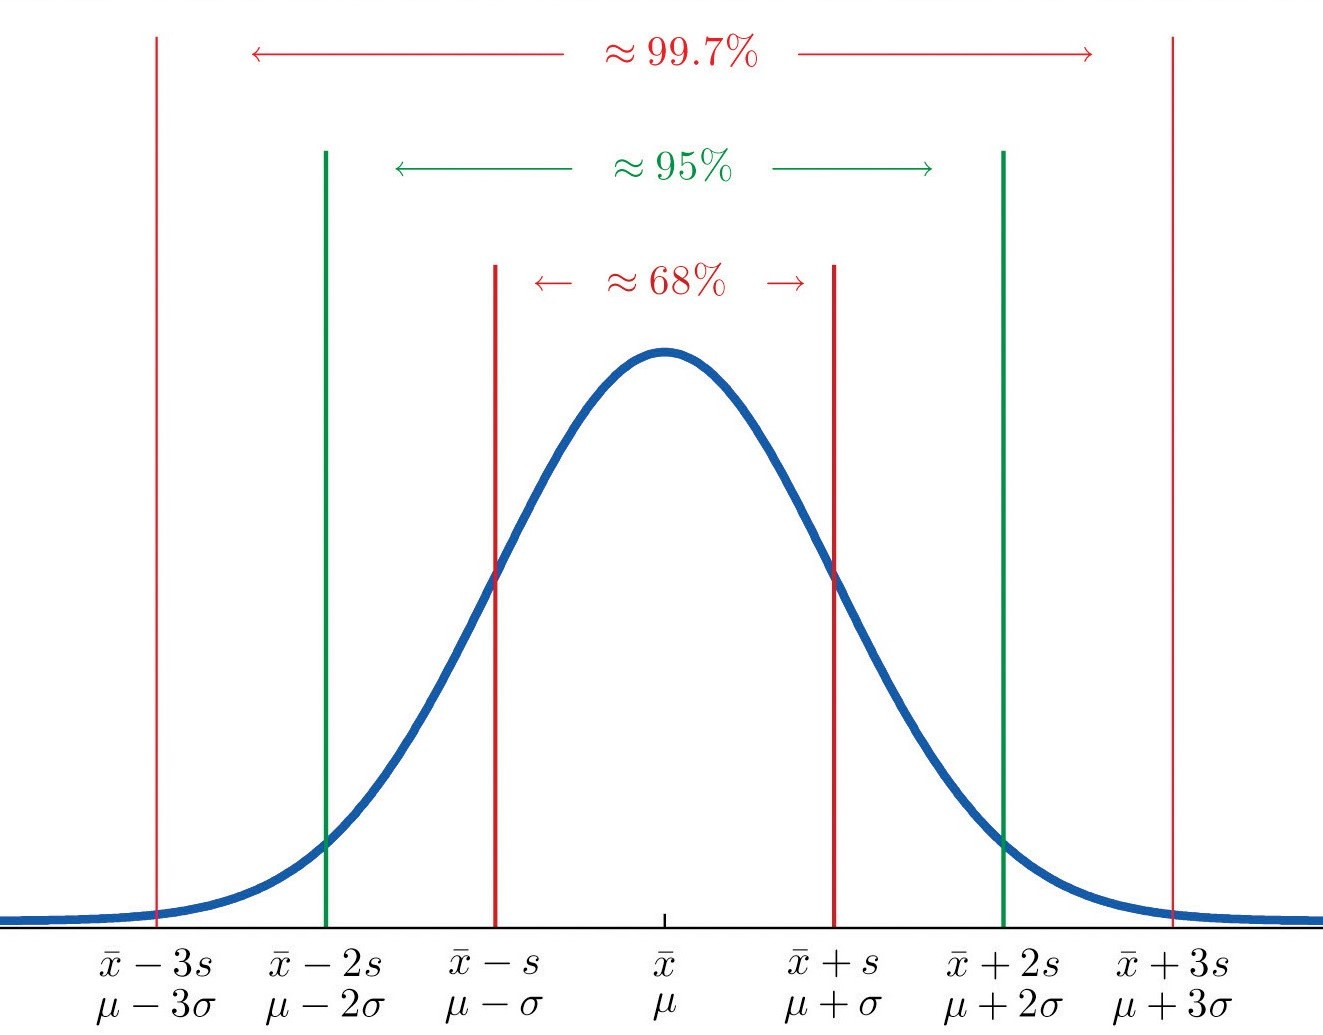
\includegraphics[width=0.9\textwidth]{Figures/Empirical-Rule.jpg}
\end{center}

\hypertarget{chebyshevs-theorem}{%
\subsection{Chebyshev's Theorem}\label{chebyshevs-theorem}}

For any numerical data set, at least \(1-1/k^2\) of the data lie within
\(k\) standard deviations of the mean, where \(k\) is any positive whole
number that is at least 2.
\begin{center}
  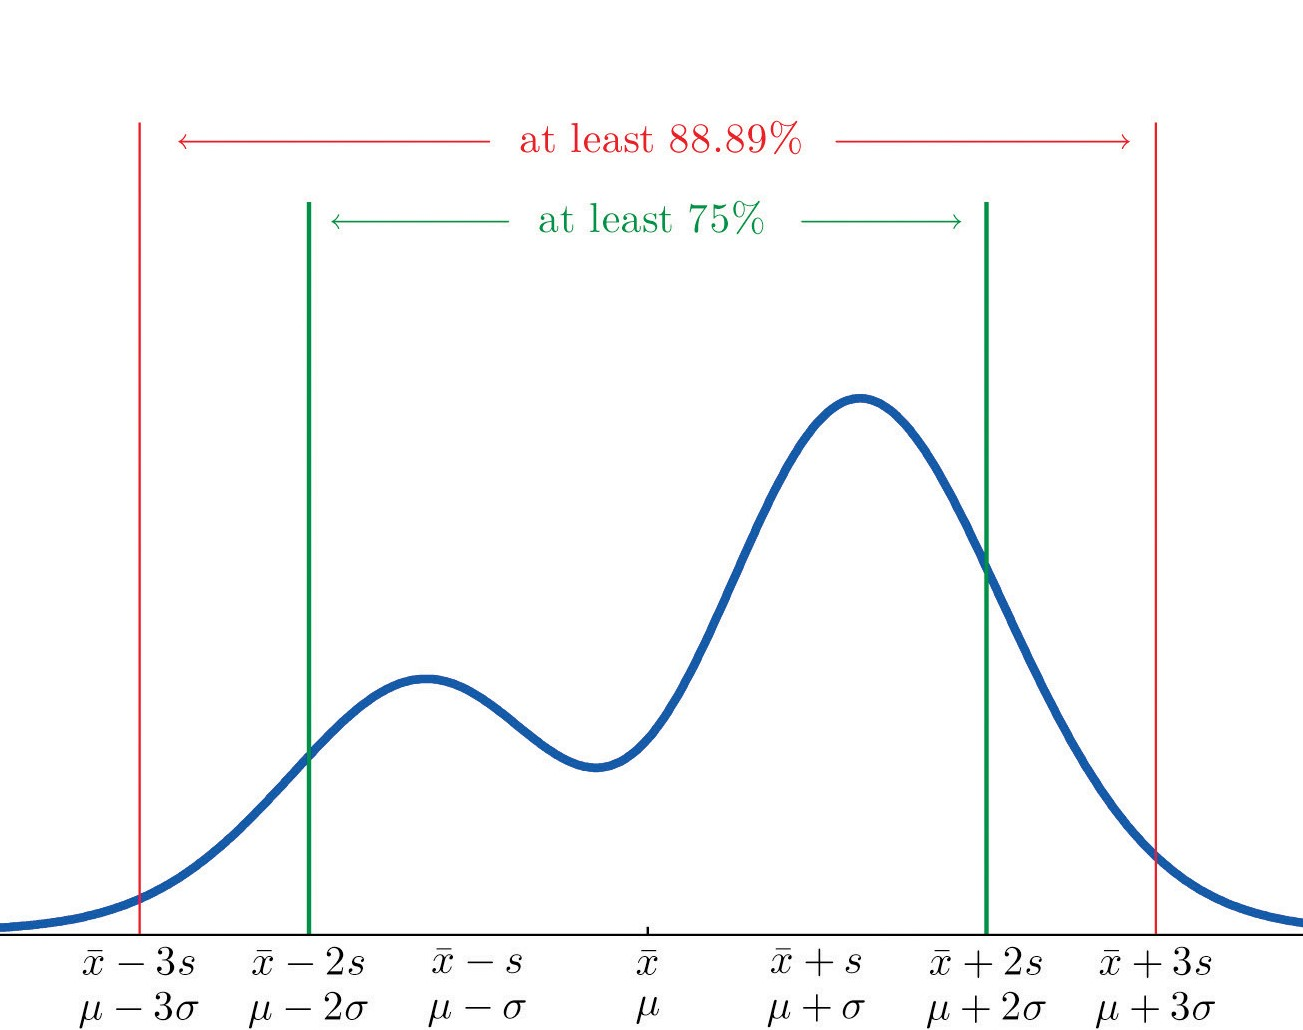
\includegraphics[width=0.9\textwidth]{Figures/Chebyshev.jpg}
\end{center}

\begin{example}

A population data set with a bell-shaped distribution has mean
\(\mu = 6\) and standard deviation \(\sigma = 2\). Find the approximate
proportion of observations in the data set that lie:

\begin{enumerate}
\item
  between 4 and 8;
\item
  below 4.
\end{enumerate}

\end{example}

\begin{example}

A sample data set has mean \(\bar{x}=6\) and standard deviation
\(s = 2\). Find the minimum proportion of observations in the data set
that must lie between 2 and 10.

\end{example}
\vspace*{6\baselineskip}

\begin{exercise}

The maintenance department at the main campus of a large state
university receives daily requests to replace fluorecent lightbulbs. The
distribution of the number of daily requests is bell-shaped and has a
mean of 60 and a standard deviation of 9. Using the 68-95-99.7 rule,
what is the approximate percentage of lightbulb replacement requests
numbering between 60 and 78?

\end{exercise}
\vspace*{6\baselineskip}

\begin{exercise}
  A sample data set has mean \(\bar{x}=10\) and standard deviation
  \(s = 3\). Find the minimum proportion of observations in the data set
  that must lie between 1 and 19.
\end{exercise}
\vspace*{6\baselineskip}

\hypertarget{more-practice}{%
\subsection{More Practice}\label{more-practice}}

\begin{exercise}

A teacher decide to curve the final exam by adding 10 points for each
student. Which of the following statistic will NOT change:
\begin{enumerate*}
  \item median, \item mean, \item interquartile range, \item standard deviation?
\end{enumerate*}
\textbf{Please explain your conclusion.}

\end{exercise}
\vspace*{6\baselineskip}

\begin{exercise}

Which distribution of data has the SMALLEST standard deviation? Please
explain your conclusion.

\begin{fullwidth}
  \begin{center}
    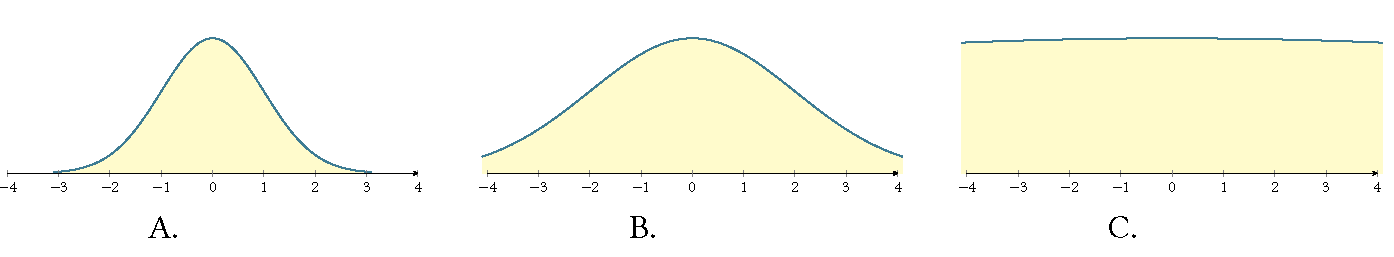
\includegraphics{Figures/SD-Pic.png}
  \end{center}
\end{fullwidth}

\end{exercise}
\vspace*{6\baselineskip}

\hypertarget{lab-3-centers-and-variations}{%
\subsection{Lab 3: Centers and
Variations}\label{lab-3-centers-and-variations}}

\hypertarget{mean-median-quartiles-and-standard-deviation}{%
\subsubsection{Mean, Median, Quartiles and Standard
Deviation}\label{mean-median-quartiles-and-standard-deviation}}

\begin{itemize}
\item
  To find the median, you may use the function \texttt{MEDIAN()}.
\item
  To find quartiles, you may use the function \texttt{QUARTILE.EXC()}.

  \textbf{Note:} this function calculates first and third quartiles with
  25\% and 75\% weights. The results may be different from the results
  calculated by hand discussed in this course.
\item
  To find the mean, you may use the function \texttt{AVERAGE()}.
\item
  To find the \textbf{population} standard deviation, you may use the
  function \texttt{STDEV.P()}.
\item
  To find the \textbf{sample} standard deviation, you may use the
  function \texttt{STDEV.S()}.
\end{itemize}

\hypertarget{how-to-create-a-boxplot-in-excel}{%
\subsubsection{How to Create a Boxplot in
Excel}\label{how-to-create-a-boxplot-in-excel}}

\begin{itemize}
\item
  Select your data---either a single data series, or multiple data
  series.
\item
  Click \texttt{Insert} $\rightarrow$ \texttt{Insert\ Statistic\ Chart}
  $\rightarrow$ \texttt{Box\ and\ Whisker} to create a boxplot.
\end{itemize}

For more information, see
\href{https://support.microsoft.com/en-us/office/create-a-box-and-whisker-chart-62f4219f-db4b-4754-aca8-4743f6190f0d}{Create
a box and whisker chart in Excel 365}

\begin{exercise}

Consider the following sample that consists of speeds of 20 cars.

19, 4, 17, 22, 23, 8, 20, 19, 10, 10, 13, 13, 15, 12, 20, 14, 9, 20, 12,
11

\begin{enumerate}[sepno]
\item
  Use Excel to find the mean, median, quartiles and standard deviation
  of the sample.
\item
  Create a box-plot for the sample.
\end{enumerate}

\end{exercise}

